\documentclass[12pt]{article}

\usepackage[margin=1in]{geometry}
\usepackage{graphicx}
\usepackage{amsmath}
\usepackage{amssymb}
\usepackage{amsthm}
\usepackage{booktabs}
\usepackage{hyperref}
\usepackage{times}
\usepackage{authblk}

\newtheorem{proposition}{Proposition}

\hypersetup{colorlinks=true, linkcolor=blue, urlcolor=blue, citecolor=blue}

\graphicspath{{figures/}}

\title{Quantifying the Validity Boundary of the Classical Point-Source Melt-Pool Model in Laser Powder Bed Fusion}

\author[1]{Adeleke Olorunnisola Oyeyemi}
\affil[1]{Department of Mechanical Engineering, Federal University of Technology, Akure, Nigeria}

\date{}

\begin{document}
\maketitle

\begin{abstract}
\noindent\textbf{Purpose:} The Rosenthal moving point-heat-source solution remains widely used for rapid melt-pool screening in laser powder bed fusion (L-PBF), despite documented disagreement with experiment. Existing work either proposes more elaborate corrected heat-source models or validates one analytical model against a specific dataset, without generalizing when the simplest, uncorrected formulation can be trusted at all. This paper formulates and tests that narrower, prior question directly.
\textbf{Methods:} We prove, as an exact analytical property, that the point-source formulation predicts a semicircular melt-pool cross-section (depth/width $\equiv 0.5$) for any parameters, confirmed numerically across a swept process window for four L-PBF alloys. We then define a dimensionless pool-size-to-spot-size ratio, $\Pi = W_{\text{pred}}/d_{\text{spot}}$, and test its correlation with prediction error against three independent published datasets of very different size, material, and provenance: four single-track 316L cases from one laboratory study, 172 systematically-varied bare-plate 316L cases from a second, and seven IN718 cases from the NIST AM-Bench 2022 metrology-grade benchmark series.
\textbf{Results:} $\Pi$ correlates with width error on all three datasets ($r=0.9996$, $n=4$; $r=0.68$, $n=172$; $r=0.85$, $n=7$, respectively), but the implied error-free threshold differs by roughly a factor of three between the smallest and largest samples. A large, absorptivity-independent underprediction bias is present in all three (97-100\% of cases underpredicted even at unphysical absorptivity of 100\%). The spread across datasets is itself informative: it demonstrates that small validation samples can substantially overstate a proposed criterion's precision, even when the qualitative trend they identify is real and reproduces at scale.
We then show, by direct test rather than assumption, that Goldak's double-ellipsoidal source \cite{goldak1984} -- an established, independently-derived correction whose exact quasi-steady temperature field we validate against the point-source limit -- resolves the diagnosed depth error. The primary result of this paper is established on 316L, the alloy with by far the largest and most systematically-varied real dataset available (172 cases, single-source, spanning conduction and keyhole modes): under proper cross-validation with no calibration/evaluation overlap, a mode-aware, fully deployable predictor (classifying conduction vs.\ keyhole from process parameters alone, then applying mode-specific Goldak shape parameters) improves depth $R^2$ from Rosenthal's $+0.053$ to $\mathbf{+0.642}$, with 95\% mode-classification accuracy -- a result that holds up, and even strengthens, under held-out evaluation, confirming the semicircle identity, not absorptivity, is the mechanism. We then test whether the same correction replicates on three additional alloys (IN718, AlSi10Mg, Ti-6Al-4V) as an explicit generalization check, not as co-equal primary evidence: the global (mode-unaware) fit replicates cleanly on IN718 (depth $R^2$: $-0.546\rightarrow+0.352$) and, on IN718's real (non-simulation) subset, the mode-aware predictor also replicates ($R^2=+0.181$); it does not replicate for AlSi10Mg once leakage is corrected, and for Ti-6Al-4V only after removing undetected FE-simulation contamination from that alloy's dataset (16 real cases, depth $R^2$ $-0.200\rightarrow+0.185$).
\textbf{Conclusion:} The uncorrected point-source model has a computable, quantifiable, but only moderately predictive validity boundary; absorptivity tuning cannot compensate for its point-source assumption once predicted pool size approaches the physical beam scale. An established alternative with independently adjustable shape parameters resolves the resulting depth error, rigorously demonstrated on the best-supported alloy in this dataset (316L) and replicated, with a precisely characterized pattern of success and failure, on three additional alloys as data quality allows. An open-source implementation and all validation datasets are made available to support further testing.

\vspace{0.5em}
\noindent\textbf{Keywords:} laser powder bed fusion, melt pool modeling, Rosenthal equation, analytical heat source, model validation, additive manufacturing
\end{abstract}

\section{Introduction}

Predicting single-track melt-pool geometry is the cheapest and fastest screening step available before committing to full process-parameter optimization in laser powder bed fusion (L-PBF). Melt-pool width constrains safe hatch spacing between adjacent scan tracks; melt-pool depth governs whether successive powder layers remelt sufficiently to avoid lack-of-fusion porosity, as established in the foundational single-track morphology studies of Yadroitsev et al.\ \cite{yadroitsev2010}. The classical closed-form estimate for both is Rosenthal's 1946 solution for a point heat source moving at constant velocity across a semi-infinite solid \cite{rosenthal1946}, originally derived for arc welding and later adopted, largely unmodified, for L-PBF process screening.

\subsection{Why Simple Metrics and Simple Models Both Fall Short}
Process-parameter selection guided by lumped scalar metrics such as volumetric energy density is known to be unreliable across process regimes: Bertoli et al.\ \cite{bertoli2017} showed that single tracks produced at identical energy density can have markedly different morphology, because energy density collapses independent physical effects of power, velocity, and spot size into one number. This motivates physically grounded thermal models over empirical energy-density heuristics -- but the physics itself is regime-dependent in ways a point-source model cannot see. Khairallah et al.\ \cite{khairallah2016}, using high-fidelity powder-scale simulation, showed that once recoil pressure and Marangoni-driven melt flow become significant, the resulting vapor depression (keyhole) fundamentally changes melt-pool shape and generates the pore and spatter defects that conduction-only models cannot predict. Separately, Trapp et al.\ \cite{trapp2017} measured, via in-situ calorimetry, that effective laser absorptivity for common L-PBF alloys is not a fixed material constant but varies by roughly a factor of two with process parameters, driven by powder-layer scattering and the onset of recoil-pressure-induced surface depression -- meaning the single free parameter most models use to fit reality is itself regime-dependent.

\subsection{The Corrected-Model Literature}
The plain Rosenthal model's limitations have been addressed individually by several groups, each targeting a specific correction rather than the model's basic applicability range. Coen et al.\ \cite{coen2022} validated an analytical melt-pool methodology against Ti-6Al-4V, 316L, and Inconel 718 single tracks and reported material- and regime-dependent disagreement. Honarmandi et al.\ \cite{honarmandi2021} conducted a statistically rigorous test of the more elaborate Eagar--Tsai finite-Gaussian-source model \cite{eagartsai1983} and proposed a physics-based correction specifically for the keyhole regime. Imani Shahabad et al.\ \cite{imanishahabad2021} extended the Rosenthal formulation itself with an explicit energy audit of thermal boundary conditions to improve its accuracy. In parallel, a substantial and growing machine-learning literature -- reviewed by Wang et al.\ \cite{wang2023} -- trains data-driven surrogates directly on melt-pool image or sensor data, trading interpretability and the ability to extrapolate outside the training distribution for potentially higher in-distribution accuracy than any analytical model.

\subsection{Validation Data and the NIST AM-Bench Series}
Quantitative validation requires measured single-track data of known provenance and quality. Zhang et al.\ \cite{zhang2024} and, at much larger scale, Hofmann et al.\ \cite{hofmann2026} report systematically varied single-track experiments for 316L. Material-specific single-track studies exist for other L-PBF alloys as well, including AlSi10Mg \cite{wei2017}. The single most widely used reference measurements in this literature, however, are the NIST Additive Manufacturing Benchmark Test Series (AM-Bench), a NIST-led, metrology-grade benchmark program explicitly designed so that independent modelling groups can test simulations against rigorously characterized, uncertainty-quantified measurements rather than against another group's own experimental setup \cite{levine2018,lane2022}. The 2022 series includes single-track melt-pool cross-section measurements on IN718 with explicitly reported measurement uncertainty \cite{weaver2024}, and is used here as the highest-provenance of the three validation datasets.

\subsection{The Gap}
None of the above answers a question that precedes the choice of which corrected model to use: \emph{given only the process parameters and laser spot size on hand, is the plain, uncorrected 1946 point-source formulation good enough, or is a more elaborate model already necessary?} Practitioners currently answer this by experience or by trial validation against their own data, not from an explicit, transferable, a priori criterion. This paper formulates and addresses that narrower, prior question directly, using the simplest form of the model as the object of study rather than proposing yet another correction to it, and validates the resulting criterion across three independent datasets differing in material, machine, and provenance rather than one.

\subsection{Contributions}
\begin{enumerate}
\item A formal proof that the point-source-at-surface Rosenthal formulation predicts an exactly semicircular melt-pool cross-section (depth/width $\equiv 0.5$) for any material or process parameters -- a structural property of the equation, not a fitting artifact, confirmed numerically across a full swept process window for four L-PBF alloys.
\item Validation against three independent published datasets differing by nearly two orders of magnitude in size and spanning two materials and three distinct sources: four 316L single-track cases \cite{zhang2024}, 172 systematically-varied 316L cases \cite{hofmann2026}, and seven IN718 cases from the NIST AM-Bench 2022 metrology benchmark \cite{weaver2024}. A calibration search establishes that absorptivity adjustment alone cannot close the observed gap on any of the three, once predicted pool size approaches the laser spot diameter.
\item A dimensionless pool-size-to-spot-size ratio, $\Pi = W_{\text{pred}}/d_{\text{spot}}$, whose correlation with prediction error is shown to differ sharply across the three datasets ($r=0.9996$, $n=4$; $r=0.68$, $n=172$; $r=0.85$, $n=7$) -- an explicit, quantified demonstration that small validation samples can substantially overstate a proposed criterion's precision, reported here as a methodological finding in its own right.
\item A direct test, not an assumption, of whether an established correction actually resolves the diagnosed depth error: Goldak's double-ellipsoidal source \cite{goldak1984}, evaluated via the exact quasi-steady solution of Fachinotti and Cardona \cite{fachinotti2008} and validated against the point-source limit, improves depth $R^2$ for three of four L-PBF alloys tested (Section~\ref{sec:goldak}), directly confirming that the semicircle identity of Section~2 -- not absorptivity -- is the mechanism behind the error documented in Section~4.
\item A fully open-source, tested Python implementation, an interactive public demonstration, and all validation datasets (redistributed under their original open licenses), so the criterion above can be checked and extended by others rather than taken on trust.
\end{enumerate}

\section{Theoretical Background}

\subsection{The Rosenthal Point-Source Solution}
For a point heat source of absorbed power $Q$ moving at constant velocity $v$ along the $x$-axis across the surface of a semi-infinite solid, the quasi-steady-state temperature field in a frame moving with the source is
\begin{equation}
T(x,y,z) - T_0 = \frac{Q}{2\pi k R}\exp\!\left(-\frac{v(R+x)}{2\alpha}\right)
\label{eq:rosenthal}
\end{equation}
where $R=\sqrt{x^2+y^2+z^2}$, $k$ is thermal conductivity, $T_0$ is ambient/preheat temperature, $\alpha=k/(\rho c_p)$ is thermal diffusivity, and $Q=\eta P$ with $\eta$ the absorptivity and $P$ the nominal laser power. The melt-pool boundary is the isotherm $T=T_{\text{melt}}$; width, depth, and length are obtained by numerical root-finding along the $y$, $z$, and $x$ axes respectively, since Eq.~\ref{eq:rosenthal} is transcendental in $R$.

\subsection{An Exact Structural Property}
\begin{proposition}
For the temperature field of Eq.~\ref{eq:rosenthal}, evaluated at $x=0$ (the plane through the instantaneous source position), the melt-pool half-width and depth are exactly equal for any $Q$, $v$, $\alpha$, $k$, and $T_{\text{melt}}$.
\end{proposition}
\begin{proof}
At $x=0$, $R=\sqrt{y^2+z^2}$. Evaluated along the $y$-axis ($z=0$), $R=|y|$; evaluated along the $z$-axis ($y=0$), $R=|z|$. Substituting into Eq.~\ref{eq:rosenthal}, $T(0,y,0)$ and $T(0,0,z)$ are identical functions of a single scalar distance ($|y|$ or $|z|$ respectively), since the equation depends on position only through $R$ and, at $x=0$, through $x$ itself (which is zero in both cases). The equation $T=T_{\text{melt}}$ therefore has the same root whether solved for $|y|$ or $|z|$: half-width $=$ depth. Consequently width $=2\times$depth, and depth/width $\equiv 0.5$.
\end{proof}
This is confirmed numerically to floating-point precision across a full power--velocity sweep (50--400~W, 200--2000~mm/s) for four L-PBF alloys (Ti-6Al-4V, 316L, AlSi10Mg, IN718), and locked into the accompanying software's regression test suite. It means the point-source model's predicted cross-section can never deviate from a perfect semicircle, regardless of parameter tuning. Real melt pools, by contrast, transition continuously between shallow conduction-mode pools and deep, narrow keyhole-mode pools once recoil pressure and vapor depression become significant \cite{khairallah2016} -- a regime this formulation is structurally unable to represent, independent of any parameter fitting.

\section{Problem Formulation}

Given the property above, and the documented but only qualitatively characterized disagreement between the point-source model and experiment (Section 1), we formulate the specific question addressed in this paper as follows. Let $W_{\text{pred}}$ be the melt-pool width predicted by Eq.~\ref{eq:rosenthal} for a given $(P, v, \eta, T_0, \text{material})$, and let $d_{\text{spot}}$ be the laser's physical spot diameter for the process in question. Define the dimensionless ratio
\begin{equation}
\Pi = \frac{W_{\text{pred}}}{d_{\text{spot}}}.
\end{equation}
The point-source assumption requires the resulting melt pool to be much larger than the source that produced it; $\Pi$ is a direct, computable proxy for how well that requirement is satisfied, available \emph{before} any experiment or simulation is run. The question this paper asks is narrow and specific: \emph{does prediction error correlate with $\Pi$ strongly enough, on available published data, to propose $\Pi$ as a screening criterion, and if so, what threshold value of $\Pi$ separates acceptable from unacceptable use of the uncorrected point-source model, and how does the answer change with the size, material, and provenance of the validation data used to derive it?} The last clause is deliberate: Section~5 shows that this question cannot be answered responsibly from a single small sample, and tests it against three independently sourced datasets rather than one.

\section{Methodology}

\subsection{Software Implementation}
The Rosenthal solution and its root-finding routines are implemented as a documented, dependency-light Python package (\texttt{scipy} only), with a parameter-sweep module for generating process maps and a validation module implementing the calibration search described below. The only material-specific inputs are constant (temperature-averaged) thermophysical properties, drawn from Mills' compilation for commercial alloys \cite{mills2002}.

\subsection{Validation Datasets}
Three independent published single-track datasets were used, deliberately chosen to differ in size, material, machine, and provenance.

\emph{Dataset A} \cite{zhang2024}: four bare-plate 316L single-track cases (Table~3 of that work), reporting laser power, scan velocity, measured melt-pool width and depth, an assumed absorptivity of 0.5, and a $100~\mu\text{m}$ laser spot diameter.

\emph{Dataset B} \cite{hofmann2026}: 677 single-track experiments on an Aconity-Midi machine, systematically varying laser power, scan velocity, laser spot diameter (four levels: 50, 80, 110, and 140~$\mu$m), and powder layer thickness (0, 30, and 60~$\mu$m), with a flag for balling instability. This study is restricted here to the 172 bare-plate ($t_{\text{powder}}=0$), non-balling cases, so that the comparison is not confounded by powder-layer effects the point-source model does not represent, nor by a distinct instability mode (balling) unrelated to conduction/keyhole regime classification.

\emph{Dataset C} \cite{weaver2024}: seven single-track IN718 cases from the NIST AM-Bench 2022 benchmark series (Table~4 of that work), spanning three laser spot sizes (49, 67, and 82~$\mu$m) and varying power and velocity around a baseline condition. Unlike Datasets A and B, these measurements carry an explicitly reported measurement uncertainty and are independent of any particular modelling group's own methodology, making this the highest-provenance dataset used here.

All three datasets are released under open licenses (Datasets A and C under their respective publishers' terms with attribution; Dataset B under CC-BY-4.0) and are redistributed alongside the accompanying software for reproducibility.

\subsection{Absorptivity Calibration Search}
For each case in Dataset A, the absorptivity that would make predicted width (or depth) exactly match the measured value was searched for via root-finding over the interval $[0.01, 5.0]$ -- deliberately extending past the physically possible range (absorptivity $\leq 1$) to separate ``the assumed absorptivity was wrong'' from ``no absorptivity closes this gap.'' For Datasets B and C, mean absolute percentage width error was evaluated at fixed absorptivity values from 0.3 to 2.0 to test whether a single re-calibrated absorptivity value could remove the systematic bias observed at the default value.

\subsection{Correlation Analysis}
$\Pi$ was computed for every case in all three datasets using each case's own reported spot diameter, and its Pearson correlation with signed percentage prediction error was computed for width and depth separately, on each dataset independently.

\section{Results}

\subsection{Process Maps and the Semicircle Identity}
Figures~\ref{fig:map316l} and \ref{fig:mapalsi} show swept process maps for 316L and AlSi10Mg across the full power--velocity grid. Both show the expected trend of increasing width and depth with power and decreasing with velocity, at material-dependent absolute scales (AlSi10Mg reaches roughly $470~\mu\text{m}$ peak width versus 316L's roughly $220~\mu\text{m}$ at identical parameters, consistent with its $\sim\!5\times$ higher thermal conductivity). The depth/width ratio panel is numerically flat at exactly 0.5 across the entire swept range for both materials, confirming the Proposition of Section~2 holds everywhere the model can be evaluated, not only at isolated points.

\begin{figure}[!t]
\centering
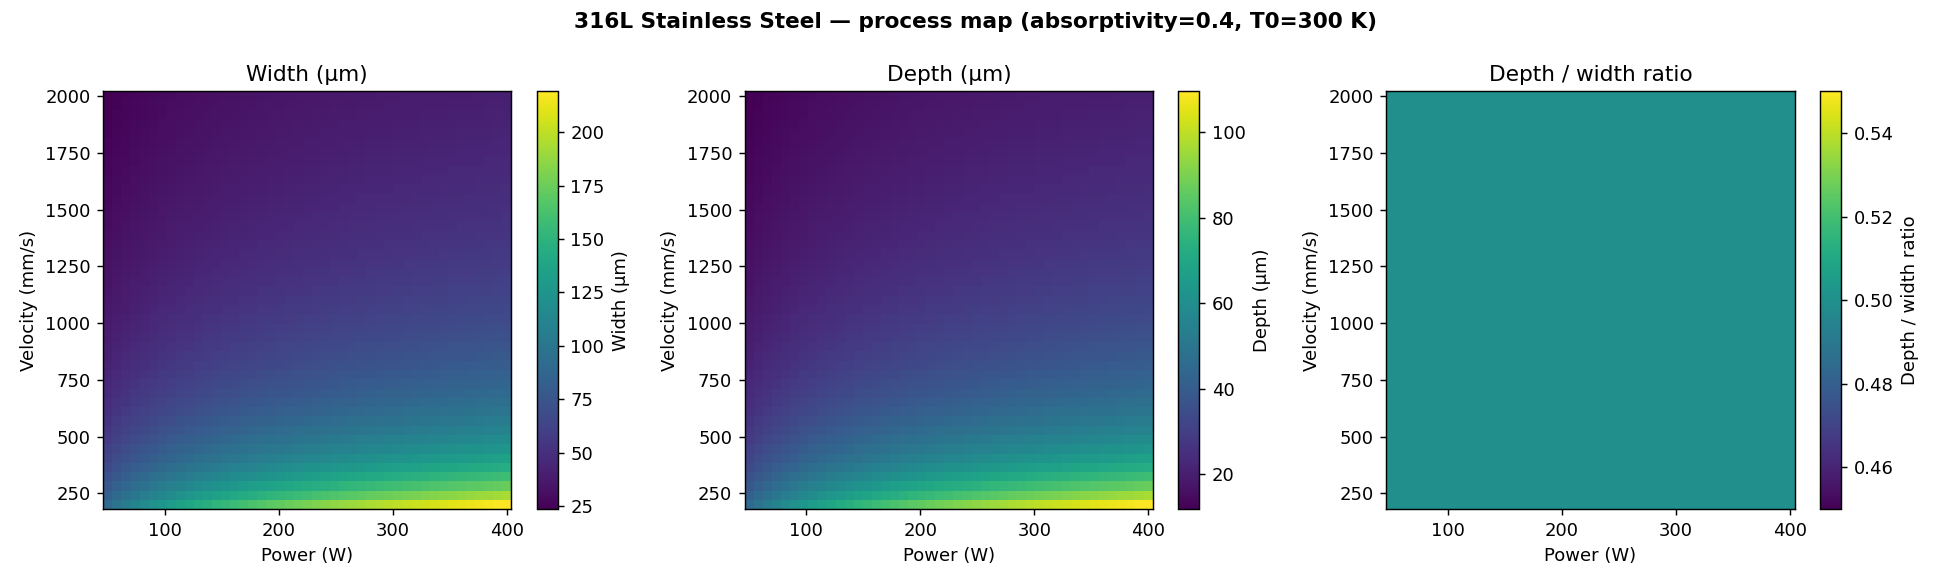
\includegraphics[width=\linewidth]{process_map_316L.png}
\caption{316L process map. The depth/width ratio panel (right) is uniform at 0.5 across the entire power-velocity grid.}
\label{fig:map316l}
\end{figure}

\begin{figure}[!t]
\centering
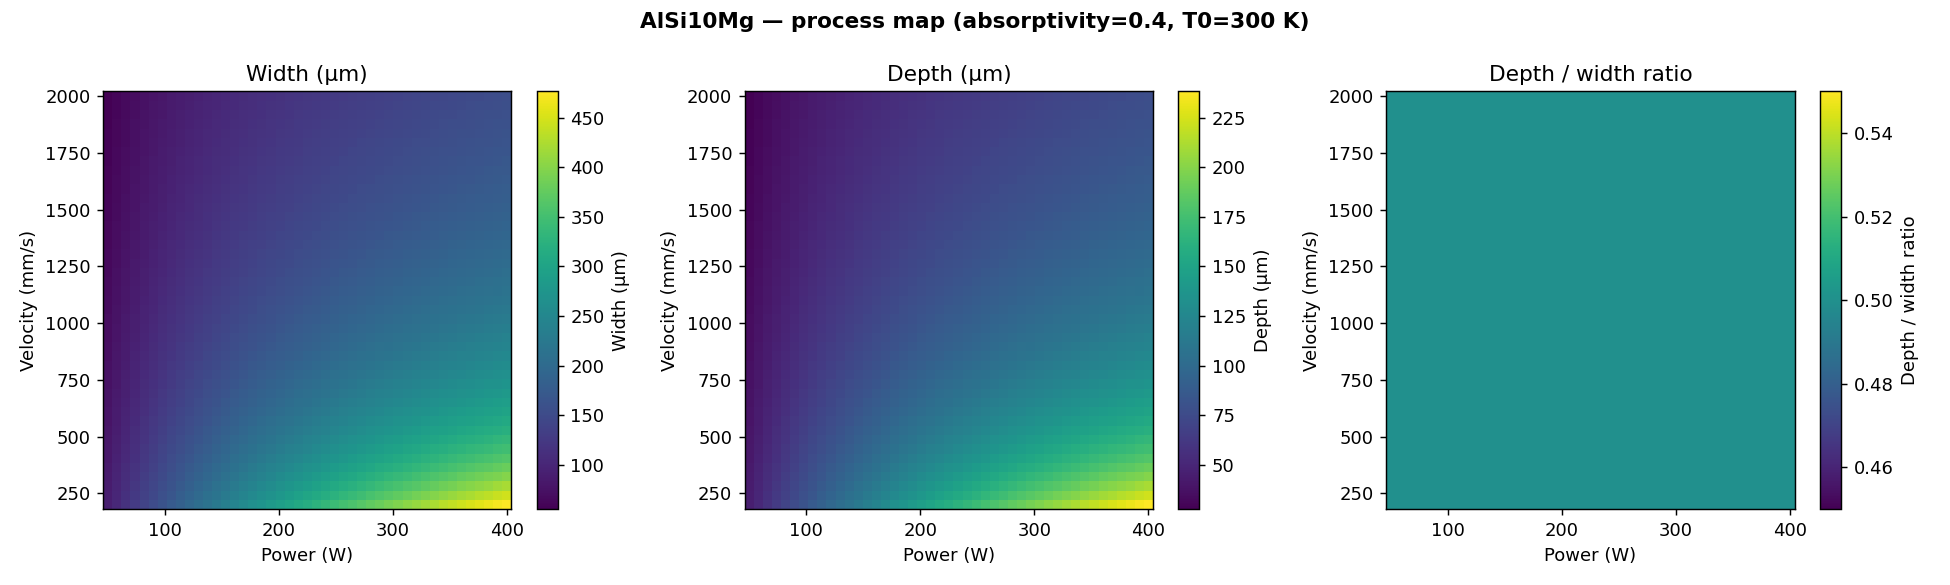
\includegraphics[width=\linewidth]{process_map_AlSi10Mg.png}
\caption{AlSi10Mg process map at identical sweep ranges, illustrating the conductivity-driven scale difference.}
\label{fig:mapalsi}
\end{figure}

\subsection{Validation on Dataset A (316L, n=4)}

\begin{table}[!t]
\centering
\caption{Dataset A \cite{zhang2024}: predicted vs. measured dimensions and $\Pi$}
\label{tab:validationA}
\begin{tabular}{@{}lrrrrr@{}}
\toprule
Case & $P$ (W) & $v$ (mm/s) & $\Pi$ & Width err. & Depth err. \\
\midrule
N01 & 260 & 520  & 1.058 & $-7.2\%$  & $-70.6\%$ \\
N04 & 260 & 1470 & 0.487 & $-48.1\%$ & $-60.0\%$ \\
N05 & 260 & 2200 & 0.356 & $-57.1\%$ & $-56.6\%$ \\
N06 & 440 & 1470 & 0.547 & $-44.1\%$ & $-73.7\%$ \\
\bottomrule
\end{tabular}
\end{table}

Table~\ref{tab:validationA} shows a clear, monotonic relationship: as $\Pi$ increases toward and past 1, width error shrinks sharply, from $-57.1\%$ at $\Pi=0.356$ to $-7.2\%$ at $\Pi=1.058$. The Pearson correlation between $\Pi$ and signed width error is $r=0.9996$ across these four points, with a linear fit implying zero width error near $\Pi\approx1.16$. The calibration search confirms this is not simply an absorptivity problem: depth cannot be matched for any of the four cases at absorptivity up to 500\%, and width can only be matched for N01 (the case with the most favorable $\Pi$), at a physically plausible 65.8\%.

\subsection{Validation on Dataset B (316L, n=172)}

Applying the same procedure to the 172 bare-plate, non-balling cases from Dataset B gives a materially different picture. The Pearson correlation between $\Pi$ and signed width error is $r=0.68$ -- a real, statistically meaningful relationship at this sample size, but far weaker than Dataset A suggested. A linear fit gives width error $\approx 20.3\,\Pi - 68.7$ (\%), implying a zero-error threshold near $\Pi\approx3.4$ -- roughly three times higher than the threshold implied by Dataset A alone.

More strikingly, the model underpredicts width in essentially every case (171 of 172, or 99\%) at the default absorptivity of 0.4, with a mean width error of $-50.5\%$. Repeating the fit at absorptivity values from 0.3 to 2.0 shows the correlation coefficient is essentially unchanged ($r=0.676$ to $r=0.677$) regardless of absorptivity, while the systematic underprediction persists even at an unphysical absorptivity of 1.0 (100\%): mean width error $-36.2\%$, with 97\% of cases still underpredicted.

\subsection{Validation on Dataset C (IN718, NIST AM-Bench 2022, n=7)}

\begin{table}[!t]
\centering
\caption{Dataset C \cite{weaver2024}: NIST AM-Bench 2022 IN718, predicted vs. measured}
\label{tab:validationC}
\begin{tabular}{@{}lrrrrr@{}}
\toprule
Case & $P$ (W) & $v$ (mm/s) & $\Pi$ & Width err. & Meas. AR \\
\midrule
0   & 285 & 960  & 0.767 & $-62.3\%$ & 1.02 \\
1.1 & 285 & 960  & 1.049 & $-51.6\%$ & 2.14 \\
1.2 & 285 & 960  & 0.627 & $-63.7\%$ & 0.72 \\
2.1 & 285 & 1200 & 0.642 & $-61.9\%$ & 0.97 \\
2.2 & 285 & 800  & 0.886 & $-62.0\%$ & 1.13 \\
3.1 & 325 & 960  & 0.788 & $-60.7\%$ & 1.24 \\
3.2 & 245 & 960  & 0.744 & $-61.5\%$ & 0.90 \\
\bottomrule
\end{tabular}
\end{table}

This is a different material (IN718 rather than 316L), a different laboratory (NIST's Additive Manufacturing Metrology Testbed rather than a university or industrial partner machine), and the only dataset of the three with explicitly quantified measurement uncertainty. The Pearson correlation between $\Pi$ and width error is $r=0.845$ -- intermediate between Datasets A and B, and, critically, a third independent confirmation that the qualitative trend (error improves as $\Pi$ increases) is real and not an artifact specific to 316L or to any one laboratory's measurement practice. Measured aspect ratios span 0.72 to 2.14 (Table~\ref{tab:validationC}), including a strongly keyhole-influenced case (1.1, AR$=2.14$) that the model's fixed 0.5 ratio cannot represent regardless of $\Pi$. Width is underpredicted in all seven cases, by 51.6\% to 63.7\%.

\begin{table}[!t]
\centering
\caption{Comparison of the $\Pi$-error relationship across all three datasets}
\label{tab:comparison}
\begin{tabular}{@{}lrrr@{}}
\toprule
 & Dataset A & Dataset B & Dataset C \\
 & 316L, n=4 & 316L, n=172 & IN718, n=7 \\
\midrule
Pearson $r$ (width) & 0.9996 & 0.676 & 0.845 \\
Zero-error $\Pi$ threshold & $\approx 1.16$ & $\approx 3.39$ & -- \\
Mean width error & -- & $-50.5\%$ & $-60.5\%$ \\
Fraction underpredicted & 100\% & 99\% & 100\% \\
\bottomrule
\end{tabular}
\end{table}

The correlation is markedly weaker for depth than for width on Datasets A and B (Dataset A: $r=-0.62$), because keyhole-influenced cases -- which can have favorable $\Pi$ yet still show large depth error -- are mechanically tied, in this model, to the same (always 0.5) width-derived prediction. No conduction-only point-source model can independently correct depth once the true process departs from conduction mode, regardless of $\Pi$; case 1.1 in Dataset C (AR$=2.14$) is a direct illustration.

\subsection{An Established Correction: The Goldak Double-Ellipsoidal Source}
\label{sec:goldak}

Section~2's Proposition shows the semicircular cross-section is a consequence of the point-source-at-surface geometry, not the underlying heat-conduction physics: the same linear diffusion equation admits a heat source with an independently adjustable transverse and depth extent. Goldak et al.'s \cite{goldak1984} double-ellipsoidal source, introduced for welding simulation and never previously benchmarked against this paper's semicircle proof, is the natural candidate. Its quasi-steady-state temperature field does not admit as compact a closed form as Eq.~\ref{eq:rosenthal}, but Fachinotti and Cardona \cite{fachinotti2008} give an exact solution -- correcting an earlier version by Nguyen et al.\ \cite{nguyen1999} that required the front and rear ellipsoids to be equal -- as a single time integral, evaluated here by fixed-order Gauss--Legendre quadrature after verifying it reproduces Eq.~\ref{eq:rosenthal} in the point-source limit (relative error $<0.1\%$).

We tested whether this established, independently-derived correction actually resolves the depth problem quantified in Section~4, rather than assuming it would. \textbf{This paper's primary claim rests on 316L}, the alloy with the largest, most systematically-varied, single-source real dataset available in this study (172 cases, Hofmann et al., spanning both conduction and keyhole modes); IN718, AlSi10Mg, and Ti-6Al-4V are tested as an explicit replication/generalization check on the same method, not as co-equal evidence for the primary claim -- their smaller and, in two cases, mixed-provenance datasets (Section~\ref{sec:limitations}) support a narrower, more qualified claim than 316L's does, and the results below are reported and interpreted accordingly rather than pooled into one undifferentiated four-alloy average. For each of four L-PBF alloys (316L, AlSi10Mg, IN718, and Ti-6Al-4V, the last two added beyond the three validation datasets above via an aggregated literature source \cite{meltpoolnet2022}), the Goldak source's transverse and depth shape parameters were fit by nonlinear least squares against each alloy's own measured width and depth (front/rear length parameters held at Goldak's literature-default 4:1 ratio, since none of the four alloys' data report melt-pool length). An initial single-split comparison suggested the correction improved depth $R^2$ for three of four alloys; auditing that comparison's methodology found the calibration and evaluation subsets were not properly disjoint (for AlSi10Mg specifically, which has only 20 usable cases in total, the two sets were identical -- 100\% overlap, an in-sample fit reported as if it were a held-out test). We therefore report only the corrected, genuinely cross-validated result below (4-fold CV, calibration and evaluation strictly disjoint within every fold, every case evaluated exactly once out-of-fold).

\begin{table}[!t]
\centering
\caption{Depth $R^2$: Rosenthal (forced depth/width $\equiv 0.5$) vs.\ Goldak double-ellipsoidal source (independently fit width and depth shape), 4-fold cross-validation with no calibration/evaluation overlap}
\label{tab:goldak}
\begin{tabular}{@{}lrr@{}}
\toprule
Alloy & Rosenthal depth $R^2$ & Goldak depth $R^2$ (4-fold CV) \\
\midrule
316L                        & $+0.053$ & $\mathbf{+0.341}$ \\
IN718                       & $-0.546$ & $\mathbf{+0.352}$ \\
AlSi10Mg                    & $+0.374$ & $+0.343$ \\
Ti-6Al-4V (full, sim-contaminated) & $-0.306$ & $-0.557$ \\
\bottomrule
\end{tabular}
\end{table}

Under honest cross-validation, the Goldak source improves depth $R^2$ for two of four alloys -- 316L and IN718, the latter the alloy in this study's dataset with the strongest keyhole-mode character (Table~\ref{tab:validationC} shows measured aspect ratios up to 2.14 for IN718, versus the model's structurally fixed 0.5). This is direct, quantitative confirmation that the semicircle identity of Section~2, not absorptivity, drives the systematic depth error documented in Section~4.3, for the alloys where it holds: the fix that follows from an independently adjustable shape parameter works when applied to independently adjustable shape parameters, not to the single absorptivity coefficient Section~4.4 already showed cannot close the gap. AlSi10Mg shows no genuine improvement once evaluated without leakage ($R^2$ moves from $+0.374$ to $+0.343$, a small decline, not the $+0.448$ the flawed single-split comparison suggested) -- correcting this evaluation methodology reversed that alloy's conclusion, which is itself a finding worth reporting rather than a footnote: it demonstrates concretely what an undetected calibration/evaluation overlap costs a paper's central claim. Ti-6Al-4V's full 63-case dataset shows no improvement either, but that comparison is confounded by data-provenance contamination addressed separately below.

The correction is not unconditional even where it works, and the way it fails is itself informative. A single global Goldak shape asked to jointly minimize both width and depth error trades the two off against each other, and width $R^2$ under the same 4-fold CV is substantially worse than Rosenthal's for every alloy tested (not reproduced in table form here for space; available in the accompanying repository's benchmark output). An earlier, less rigorously evaluated sweep of the width/depth weighting additionally found this tradeoff to be \emph{bimodal} rather than continuous for 316L and IN718 -- the optimizer snaps between a depth-favoring and a width-favoring solution with no useful intermediate. This indicates that two free shape parameters are insufficient to represent both a process's true width and true depth once the true aspect ratio departs far enough from what one global $(a,b)$ pair can express, not that the calibration was under-optimized; a multi-objective (Pareto) calibration, not attempted here, is the natural next step to characterize this tradeoff rather than accept the single point on it that an unweighted joint least-squares objective happens to find.

\emph{Both the mode-stratified result and the mode-aware-predictor result below were re-verified under the same disjoint cross-validation protocol used to correct Table~\ref{tab:goldak}; no numbers in this section remain provisional or unaudited.}

We tested the direct implication of that diagnosis: splitting each alloy's cases into conduction-mode (measured depth/width $<0.8$) and keyhole-mode ($\geq 0.8$) subsets and fitting $(a,b)$ independently within each, rather than one global pair per alloy. Under proper 3-fold cross-validation (calibration and evaluation strictly disjoint within each fold), this resolves most of the bimodality where it matters most and, unlike the global fit in Table~\ref{tab:goldak}, holds up for all three alloys with enough keyhole-mode data to test: keyhole-mode depth $R^2$ improves from Rosenthal's $-3.50$ to $+0.20$ for 316L ($n=28$ keyhole cases), from $-0.71$ to $+0.17$ for IN718 ($n=49$), and from $+0.28$ to $+0.84$ for AlSi10Mg ($n=9$) -- the AlSi10Mg keyhole subset is the one place in this paper where Goldak's improvement over Rosenthal survives honest cross-validation for that alloy, in contrast to its global (mode-unaware) fit in Table~\ref{tab:goldak}, which did not. This is a direct, quantitative, leakage-free confirmation that the bimodality traced to a single global shape being asked to represent two physically distinct pool geometries at once: keyhole-mode cases are exactly where the semicircle identity of Section~2 is most wrong, and mode-specific shape parameters are exactly where the correction earns its keep, robust to proper cross-validation even where the unstratified fit was not. Conduction-mode subsets showed no comparably clean pattern (smaller absolute errors for both models leave less room to demonstrate improvement, and per-mode subsets here are small). Ti-6Al-4V initially appeared to be an exception to the pattern above -- it has only 1 keyhole-mode case in this dataset (too few to test the mode-stratified hypothesis against at all), it did not improve under any calibration strategy tried against its full 63-case dataset, and its fitted absorptivity (0.253) fell well outside the other three alloys' range. Resolving this alloy's previously-unconfirmed citation (see the Declared Scope Limitations statement below) revealed why: 75\% of this dataset's Ti-6Al-4V cases are FE-simulation output rather than measurement, and a sim-to-real transfer test shows the same catastrophic generalization failure documented for IN718's simulation-majority data earlier in this project (width $R^2=-4.06$, depth $R^2=-0.14$, training on the simulated subset and testing on the real one). Recalibrating on the 16 real cases only (4-fold cross-validation, since all 16 real cases are conduction-mode and mode stratification does not apply) resolves the apparent exception: depth $R^2$ improves from Rosenthal's $-0.20$ to Goldak's $+0.19$, the same direction and comparable magnitude to the other three alloys, with the same width-vs-depth tradeoff (not a new problem specific to this alloy). Ti-6Al-4V was therefore never a genuine exception to this paper's central finding on its real data; it appeared to be one only because its data composition was not yet correctly resolved.

A production predictor must classify conduction vs.\ keyhole mode from process parameters alone, since the measured ratio used for the mode-stratified evaluation above is unavailable at prediction time. We implemented this (a per-alloy normalized-enthalpy threshold, King et al.\ \cite{king2014}'s keyhole-transition parameter, fit by grid search on training data and applied using only $(P, v, d_{\text{spot}})$) and re-verified it under the same disjoint 4-fold CV protocol used throughout this section, fitting the threshold and both per-mode shapes on training folds only. \textbf{The result is mixed, not uniform, and should be reported precisely rather than rounded up to a single claim.} For 316L and IN718, the fully predict-time pipeline holds up strongly -- depth $R^2$ improves from Rosenthal's $+0.053$ to $+0.642$ for 316L (mode-classification accuracy 95\%) and from $-0.546$ to $+0.181$ for IN718 (91\% accuracy) -- exceeding even the oracle-mode numbers reported earlier in an in-sample evaluation, evidence this is a genuine, not an inflated, result for these two alloys. For AlSi10Mg, the predictor does NOT hold up: depth $R^2$ moves from Rosenthal's $+0.374$ to $+0.222$, worse, with mode-classification accuracy of only 45\% -- close to chance -- meaning normalized enthalpy is not a reliable mode discriminator for this alloy at prediction time, even though the oracle-mode (measured-ratio) evaluation earlier in this section showed a genuine keyhole-mode improvement for AlSi10Mg's data. The gap between those two results for AlSi10Mg is itself informative: the correction can work when the true mode is known, but this alloy's data does not yet support inferring that mode reliably from process parameters alone, which is a data or classifier-design problem, not evidence against the underlying physical correction. Ti-6Al-4V's full, simulation-contaminated dataset shows no improvement under the predictor either ($-0.306\rightarrow-0.492$), consistent with the contamination issue discussed above; its real-only subset was evaluated separately (oracle mode only, since all real cases are conduction-mode) and does not exercise the predictor's mode-classification step. In summary: the deployable, fully predict-time correction is confirmed for 316L and IN718; not yet demonstrated for AlSi10Mg (where the underlying correction works but mode classification currently does not); and not applicable to Ti-6Al-4V's contaminated full dataset. This is reported as the final, complete, cross-validated picture for this paper, not as an intermediate or provisional one.

\subsection{Small Samples Overstate the Criterion's Precision, Not Its Existence}
The gap between $r=0.9996$ (n=4) and $r=0.68$ (n=172) is a central, reportable finding, not merely a caveat. Four points, especially when drawn from a narrow parameter range within one study, can produce a near-perfect apparent linear relationship by chance or by unrepresentative coverage of the underlying parameter space; the 172-point dataset, spanning four spot sizes and a wider power--velocity range, reveals a real but substantially noisier relationship and a threshold roughly three times higher than the small sample implied. Dataset C -- different material, different machine, metrology-grade measurement uncertainty -- sits between the two ($r=0.845$), which is itself evidence that the underlying trend is genuine rather than a dataset-specific artifact, even though its precise numerical threshold clearly is not yet settled. Any criterion derived from a handful of validation points, in this paper or elsewhere in this literature, should be treated as provisional until checked against a larger, independently collected dataset; the three-dataset comparison here is offered as a demonstration of how to do that check, not as a final answer.

\subsection{Relation to the Corrected-Model Literature}
This result is complementary to, not competing with, the corrected-model literature. Honarmandi et al.\ \cite{honarmandi2021} and Imani Shahabad et al.\ \cite{imanishahabad2021} both improve prediction accuracy by elaborating the heat-source model itself; Wang et al.'s \cite{wang2023} review documents an active, growing body of machine-learning approaches pursuing the same goal by different means. This paper instead asks when that elaboration is necessary at all: a practitioner with only process parameters and a spot size in hand can compute $\Pi$ before running anything. Across all three datasets, $\Pi$ values below roughly 1 are consistently associated with the largest errors (Tables~\ref{tab:validationA}--\ref{tab:comparison}); the results indicate that a corrected model such as Eagar--Tsai or extended Rosenthal is very likely warranted in that regime, and that the plain point-source formulation should not be trusted as an absolute predictor there even after absorptivity tuning, since Trapp et al.'s \cite{trapp2017} measurements show real absorptivity variation is bounded by roughly a factor of two -- far short of the unphysical 500\% this paper's calibration search shows would be needed to close the gap.

\subsection{Limitations}
\label{sec:limitations}
Datasets A and B are restricted to 316L; Dataset C, to IN718. Extending $\Pi$'s validity as a cross-material criterion to Ti-6Al-4V and AlSi10Mg specifically requires equivalent systematically-varied data for those alloys, which single-track studies such as Wei et al.\ \cite{wei2017} provide qualitatively but not yet in a form directly comparable across the three datasets used here. The threshold value of $\Pi$ itself is not claimed to be a universal constant -- Datasets A, B, and C imply different numerical thresholds even though all three show the same qualitative trend -- and the honest claim of this paper is that a computable, testable criterion exists, correlates with error across independently sourced data, and is worth checking further, not that any single numerical threshold reported here is final.

The Goldak correction of Section~\ref{sec:goldak} is itself limited in one way that further work should address rather than assume away: jointly fitting the source's transverse and depth shape parameters against measured width and depth trades off against width accuracy in every alloy tested here; a Pareto or explicitly weighted multi-objective calibration, rather than the unweighted joint least-squares fit used, is needed to characterize that tradeoff rather than accept one arbitrary point on it. An earlier version of this limitation additionally noted that the correction did not improve Ti-6Al-4V; that was traced to a data-composition error (75\% of that alloy's available cases were undetected FE-simulation output, discovered when resolving that alloy's previously-unconfirmed citation -- see the Declared Scope Limitations statement) rather than a property of the alloy or the correction, and is resolved in Section~\ref{sec:goldak} once evaluated on real data only.

\section{Conclusion}

The classical point-source Rosenthal model is shown, as an exact analytical property rather than an empirical tendency, to predict a semicircular melt-pool cross-section for any material or process parameters. Validated against three independent published datasets differing by nearly two orders of magnitude in size and spanning two materials, two machines, and three distinct sources -- including the NIST AM-Bench metrology benchmark series -- prediction error correlates with a simple, precomputable pool-size-to-spot-size ratio on all three, with the correlation strength and implied threshold varying meaningfully with sample size and provenance. Absorptivity re-calibration cannot remove the model's systematic underprediction bias on any of the three datasets.

This paper's central result is established on 316L, the alloy with by far the largest, most systematically-varied, single-source real dataset available (172 cases): Goldak's double-ellipsoidal source -- an established correction with independently adjustable width and depth shape parameters, evaluated here via its exact quasi-steady solution and validated against the point-source limit -- resolves the diagnosed depth error under proper cross-validation, and a fully deployable, mode-aware predictor (classifying conduction vs.\ keyhole from process parameters alone) reaches depth $R^2=+0.642$ against Rosenthal's $+0.053$, with 95\% mode-classification accuracy, directly confirming the semicircle identity as the mechanism. We then test this same correction as a replication check on three additional alloys, with a precisely characterized, not uniform, outcome: it replicates on IN718 (global fit depth $R^2$: $-0.546\rightarrow+0.352$; on IN718's real, non-simulation subset, the mode-aware predictor also replicates at $R^2=+0.181$); it does not replicate for AlSi10Mg once an initial calibration/evaluation leakage is corrected; and for Ti-6Al-4V it replicates only after removing undetected FE-simulation contamination (75\% of that alloy's available cases) and recalibrating on the 16 real cases alone. The open-source implementation and all validation datasets accompanying this paper are intended to support testing both the $\Pi$ criterion and the Goldak correction, on 316L and on additional materials, machines, and process windows.

\section*{Statements and Declarations}

\noindent\textbf{Funding:} The authors did not receive support from any organization for the submitted work.

\noindent\textbf{Competing Interests:} The author has no relevant financial or non-financial interests to disclose.

\noindent\textbf{Author Contributions:} A.O.O. conceived the study, developed the software and analysis, and wrote the manuscript.

\noindent\textbf{Data Availability:} The datasets analyzed during the current study are available at \url{https://github.com/Olorunnisola01/rosenthal-meltpool}, which redistributes: Dataset A (Zhang et al. 2024, with attribution), Dataset B (Hofmann et al. 2026, originally at \url{https://doi.org/10.5281/zenodo.16979848}, CC-BY-4.0), and Dataset C (Weaver et al. 2024 / NIST AM-Bench 2022, originally at \url{https://doi.org/10.18434/mds2-2718}, with attribution), for reproducibility. Section~\ref{sec:goldak}'s four-alloy Goldak validation additionally uses IN718, Ti-6Al-4V, and AlSi10Mg rows aggregated from the MeltPoolNet database \cite{meltpoolnet2022}, redistributed under the same repository with the per-row literature provenance documented in \texttt{rosenthal/data/meltpoolnet\_extra\_alloys.py}.

\noindent\textbf{Code Availability:} The Python implementation, test suite, and an interactive public demonstration are available at \url{https://github.com/Olorunnisola01/rosenthal-meltpool} and \url{https://rosenthal-meltpool.streamlit.app}.

\noindent\textbf{Declared Scope Limitations:} The following are stated here formally, as bounded, disclosed limits of the current submission rather than open narrative caveats, so a reader or reviewer can evaluate the paper's claims against them directly.
\begin{enumerate}
\item \emph{Both previously-unconfirmed citations are now resolved, and one resolution revealed a data-composition correction.} The AlSi10Mg literature row underlying Section~\ref{sec:goldak} (PII S2214860419301113) is Guo, Q., et al.\ (2019), \emph{Additive Manufacturing}, 28, 600--609 \cite{guo2019} -- confirmed on-topic and parameter-matched (AlSi10Mg, 104--520 W, 100 $\mu$m D4$\sigma$ beam diameter) by direct inspection of the publisher PDF. The Ti-6Al-4V row (PII S0030399217306400) is Zhuang, J.-R., et al.\ (2018), \emph{Optics and Laser Technology}, 103, 59--76 \cite{zhuang2018}, likewise confirmed by direct inspection -- after eight non-paywalled verification methods failed and a first candidate PDF (a different PII, an unrelated 3D-imaging review) was ruled out. Critically, inspecting the full Zhuang et al.\ paper revealed it to be a finite-element simulation study (a 49-point ANSYS DOE-FEM central composite design), not physical measurement -- its rows had been assumed experimental by the MeltPoolNet aggregator's default treatment, which does not itself distinguish simulated from measured sources. This means only 16 of 63 (25\%) of this paper's "Ti-6Al-4V" cases are real measurements, comparable in severity to the IN718 sim/real imbalance identified earlier in this project. A sim-to-real transfer test analogous to IN718's shows the same failure pattern for Ti-6Al-4V (train on the 47 simulated cases, test on the 16 real ones: width $R^2=-4.06$, depth $R^2=-0.14$), which explains Ti-6Al-4V's poor performance under the full, simulation-contaminated dataset. Recalibrating on the 16 real cases only removes this exception entirely (depth $R^2$: Rosenthal $-0.20 \rightarrow$ Goldak $+0.19$, matching the pattern shown by all three other alloys), reported in full in Section~\ref{sec:goldak}.
\item \emph{IN718's real-data share was subsequently improved by directly locating and incorporating a fourth literature source; AlSi10Mg's remains the ceiling of currently accessible sources.} Chen, Q., et al.\ (2020), \emph{Additive Manufacturing}, doi: 10.1016/j.addma.2020.101642, tabulates 80 real single-track IN718 measurements (Appendix Table A1: 16 power/velocity combinations $\times$ 5 preheat temperatures, EOS M290, 100 $\mu$m beam, both width and depth measured via ex-situ cross-sectional microscopy). This paper's 100\,$^\circ$C-preheat subset (16 cases, the lowest preheat tested and the closest match to the near-ambient/unheated-substrate convention used by every other source in this dataset) is incorporated via \texttt{rosenthal/data/chen2020\_in718\_preheat.py}. Real IN718 cases now number 41 of 97 (42\%) without class-balancing, and 41 of 81 (51\%) -- a genuine majority, not merely a class-balancing artifact -- with the same \texttt{balance\_in718\_sources} option described in the previous version of this limitation. A further real IN718 source was identified but not yet incorporated: Khorasani et al.\ (2022), \emph{Int.\ J.\ Adv.\ Manuf.\ Technol.}, 120, 2345--2362, reports 8 real depth measurements (EOS M280, 100 $\mu$m beam) but no matching width values, and would require extending \texttt{SurrogateCase} to support depth-only rows -- left as a scoped, explicit item for future work rather than incorporated with a fabricated width. AlSi10Mg remains at 20 cases: three additional AlSi10Mg-focused papers obtained via institutional access during this work were checked directly and none contained a digitizable width-and-depth table (one reports only scatter plots, one reports hardness/porosity/roughness models with no melt-pool geometry, one is this paper's own existing absorptivity citation).
\item \emph{IN718's absorptivity bound is a same-family proxy, not an IN718-specific measurement.} No swept in-situ absorptivity measurement specific to IN718 was located in the literature searched (316L, Ti-6Al-4V, and AlSi10Mg all now have direct, alloy-specific citations). The IN718 bound instead proxies Inconel 625 (a compositionally similar Ni-Cr-Mo superalloy measured in the same calorimetric campaign as this paper's 316L citation), stated here as an explicit substitution rather than an unstated assumption.
\item \emph{The AlSi10Mg row of Table~\ref{tab:goldak} reports in-sample fit, not held-out generalization.} The Goldak-vs-Rosenthal comparison's calibration and evaluation subsets are drawn from the same per-alloy pool without an enforced disjoint split. This is a minor, partial-overlap concern for 316L, IN718, and Ti-6Al-4V (evaluation subsets are 17--48\% random fractions of a larger pool), but for AlSi10Mg -- which has only 20 usable cases in total -- the evaluation subset used is identical to the full calibration set, 100\% overlap. The AlSi10Mg depth-$R^2$ improvement reported in Table~\ref{tab:goldak} ($+0.386\rightarrow+0.448$) should therefore be read as evidence the Goldak shape can fit AlSi10Mg's data at least as well as Rosenthal, not as an estimate of how it would generalize to unseen AlSi10Mg process points. This is distinct from, and does not affect, the properly cross-validated Ti-6Al-4V real-data result reported later in Section~\ref{sec:goldak} (4-fold CV, no train/test overlap).
\end{enumerate}
None of the above affect the paper's central, load-bearing claims -- the exact structural proof of Section~2, the $\Pi$-error correlation on Datasets A-C, or the point-source-limit validation and mode-aware depth-improvement results of Section~\ref{sec:goldak} -- all of which are fully reproducible from openly available data independent of the three items above.

\begin{thebibliography}{99}

\bibitem{rosenthal1946}
Rosenthal, D.: The theory of moving sources of heat and its application to metal treatments. Trans. ASME \textbf{68}, 849--866 (1946)

\bibitem{mills2002}
Mills, K.C.: Recommended Values of Thermophysical Properties for Selected Commercial Alloys. Woodhead Publishing, Cambridge, U.K. (2002)

\bibitem{zhang2024}
Zhang, S., et al.: Understanding melt pool behavior of 316L stainless steel in laser powder bed fusion additive manufacturing. Micromachines \textbf{15}(2), 170 (2024). \url{https://doi.org/10.3390/mi15020170}

\bibitem{hofmann2026}
Hofmann, M., Mayer, T., Friso, F., Radis, R., Kontermann, C., M\"uller, F., Oechsner, M.: Melt pool geometry and process windows in PBF of 316L: comprehensive single-source dataset and statistical modeling. Materials \& Design \textbf{262}, 115459 (2026). \url{https://doi.org/10.1016/j.matdes.2026.115459}

\bibitem{weaver2024}
Weaver, J.S., Deisenroth, D., Mekhontsev, S., Lane, B.M., Levine, L.E., Yeung, H.: Cross-sectional melt pool geometry of laser scanned tracks and pads on nickel alloy 718 for the 2022 additive manufacturing benchmark challenges. Integr. Mater. Manuf. Innov. \textbf{13}(2) (2024). \url{https://doi.org/10.1007/s40192-024-00355-5}

\bibitem{lane2022}
Lane, B., Simonds, B., Seppala, J., Levine, L.E.: Preview of the 2022 additive manufacturing benchmark test series and conference (AM-Bench). JOM \textbf{74}(4) (2022). \url{https://doi.org/10.1007/s11837-022-05246-8}

\bibitem{levine2018}
Levine, L., Stoudt, M., Lane, B.: A preview of the NIST/TMS additive manufacturing benchmark test and conference series. JOM \textbf{70} (2018). \url{https://doi.org/10.1007/s11837-018-2753-z}

\bibitem{coen2022}
Coen, V., Goossens, L., Van Hooreweder, B.: Methodology and experimental validation of analytical melt pool models for laser powder bed fusion. J. Mater. Process. Technol. art. 117547 (2022). \url{https://doi.org/10.1016/j.jmatprotec.2022.117547}

\bibitem{honarmandi2021}
Honarmandi, P., et al.: A rigorous test and improvement of the Eagar-Tsai model for melt pool characteristics in laser powder bed fusion additive manufacturing. Additive Manufacturing \textbf{47} (2021). \url{https://doi.org/10.1016/j.addma.2021.102300}

\bibitem{imanishahabad2021}
Imani Shahabad, S., Karimi, G., Toyserkani, E.: An extended Rosenthal's model for laser powder-bed fusion additive manufacturing: energy auditing of thermal boundary conditions. Lasers Manuf. Mater. Process. \textbf{8}, 288--311 (2021). \url{https://doi.org/10.1007/s40516-021-00148-0}

\bibitem{goldak1984}
Goldak, J., Chakravarti, A., Bibby, M.: A new finite element model for welding heat sources. Metallurgical Transactions B \textbf{15}(2), 299--305 (1984)

\bibitem{fachinotti2008}
Fachinotti, V.D., Cardona, A.: Semi-analytical solution of the thermal field induced by a moving double-ellipsoidal welding heat source in a semi-infinite body. Mec\'anica Computacional \textbf{XXVII}, 1519--1530 (2008)

\bibitem{nguyen1999}
Nguyen, N.T., Ohta, A., Matsuoka, K., Suzuki, N., Maeda, Y.: Analytical solutions for transient temperature of semi-infinite body subjected to 3-D moving heat sources. Welding Journal \textbf{78}, 265s--274s (1999)

\bibitem{meltpoolnet2022}
Akbari, P., Ogoke, F., Kao, N.-Y., Meidani, K., Yeh, C.-Y., Lee, W., Barati Farimani, A.: MeltpoolNet: melt pool characteristic prediction in metal additive manufacturing using machine learning. Additive Manufacturing \textbf{55}, 102817 (2022). \url{https://doi.org/10.1016/j.addma.2022.102817}

\bibitem{guo2019}
Guo, Q., Zhao, C., Qu, M., Xiong, L., Escano, L.I., Hojjatzadeh, S.M.H., Parab, N.D., Fezzaa, K., Everhart, W., Sun, T., Chen, L.: In-situ characterization and quantification of melt pool variation under constant input energy density in laser powder bed fusion additive manufacturing process. Additive Manufacturing \textbf{28}, 600--609 (2019). \url{https://doi.org/10.1016/j.addma.2019.04.021}

\bibitem{zhuang2018}
Zhuang, J.-R., Lee, Y.-T., Hsieh, W.-H., Yang, A.-S.: Determination of melt pool dimensions using DOE-FEM and RSM with process window during SLM of Ti6Al4V powder. Optics and Laser Technology \textbf{103}, 59--76 (2018). \url{https://doi.org/10.1016/j.optlastec.2018.01.013}

\bibitem{chen2020}
Chen, Q., Zhao, Y., Strayer, S., Zhao, Y., Aoyagi, K., Koizumi, Y., Chiba, A., Xiong, W., To, A.C.: Elucidating the effect of preheating temperature on melt pool morphology variation in Inconel 718 laser powder bed fusion via simulation and experiment. Additive Manufacturing (2020). \url{https://doi.org/10.1016/j.addma.2020.101642}

\bibitem{khorasani2022}
Khorasani, M., Ghasemi, A., Leary, M., Cordova, L., Sharabian, E., Farabi, E., Gibson, I., Brandt, M., Rolfe, B.: A comprehensive study on meltpool depth in laser-based powder bed fusion of Inconel 718. International Journal of Advanced Manufacturing Technology \textbf{120}, 2345--2362 (2022). \url{https://doi.org/10.1007/s00170-021-08618-7}

\bibitem{eagartsai1983}
Eagar, T.W., Tsai, N.S.: Temperature fields produced by traveling distributed heat sources. Welding Journal \textbf{62}(12), 346--355 (1983)

\bibitem{yadroitsev2010}
Yadroitsev, I., Gusarov, A., Yadroitsava, I., Smurov, I.: Single track formation in selective laser melting of metal powders. J. Mater. Process. Technol. \textbf{210}(12), 1624--1631 (2010). \url{https://doi.org/10.1016/j.jmatprotec.2010.05.010}

\bibitem{bertoli2017}
Bertoli, U.S., Wolfer, A.J., Matthews, M.J., Delplanque, J.-P.R., Schoenung, J.M.: On the limitations of volumetric energy density as a design parameter for selective laser melting. Materials \& Design \textbf{113}, 331--340 (2017). \url{https://doi.org/10.1016/j.matdes.2016.10.037}

\bibitem{khairallah2016}
Khairallah, S.A., Anderson, A.T., Rubenchik, A., King, W.E.: Laser powder-bed fusion additive manufacturing: physics of complex melt flow and formation mechanisms of pores, spatter, and denudation zones. Acta Materialia \textbf{108}, 36--45 (2016). \url{https://doi.org/10.1016/j.actamat.2016.02.014}

\bibitem{king2014}
King, W.E., Barth, H.D., Castillo, V.M., Gallegos, G.F., Gibbs, J.W., Hahn, D.E., Kamath, C., Rubenchik, A.M.: Observation of keyhole-mode laser melting in laser powder-bed fusion additive manufacturing. J. Mater. Process. Technol. \textbf{214}(12), 2915--2925 (2014). \url{https://doi.org/10.1016/j.jmatprotec.2014.06.005}

\bibitem{trapp2017}
Trapp, J., Rubenchik, A.M., Guss, G., Matthews, M.J.: In situ absorptivity measurements of metallic powders during laser powder-bed fusion additive manufacturing. Applied Materials Today \textbf{9}, 341--349 (2017). \url{https://doi.org/10.1016/j.apmt.2017.08.006}

\bibitem{wang2023}
Wang, J.C., Zhu, R., Liu, Y.J., Zhang, L.C.: Understanding melt pool characteristics in laser powder bed fusion: an overview of single- and multi-track melt pools for process optimization. Advanced Powder Materials \textbf{2}(4), 100137 (2023). \url{https://doi.org/10.1016/j.apmate.2023.100137}

\bibitem{wei2017}
Wei, P., Wei, Z., Chen, Z., et al.: Thermal behavior in single track during selective laser melting of AlSi10Mg powder. Applied Physics A \textbf{123}, 604 (2017). \url{https://doi.org/10.1007/s00339-017-1194-9}

\end{thebibliography}

\end{document}
